% Scientific Reports manuscript (standard 'article' class, as the journal's LaTeX guidance allows).
% Build: pdflatex neurosafe_scirep.tex (twice). References are inside this file (no .bib), as required.
\documentclass[10pt,a4paper]{article}
\usepackage[utf8]{inputenc}
\usepackage[T1]{fontenc}
\usepackage{lmodern}
\usepackage[margin=2.2cm]{geometry}
\usepackage{amsmath,amssymb,amsthm,booktabs,graphicx,xcolor,url}
\usepackage[numbers,square,sort&compress]{natbib}
\usepackage{tikz}
\usetikzlibrary{positioning,arrows.meta,fit,backgrounds,calc}
\usepackage{lineno}
\usepackage[hidelinks]{hyperref}
\linenumbers
\setlength{\parskip}{3pt}
\newtheorem{theorem}{Theorem}
\newtheorem{corollary}{Corollary}
\newtheorem{definition}{Definition}
\newtheorem{proposition}{Proposition}
\renewcommand{\figurename}{Figure}
% ---- Items still to confirm before submission (shown in red). When an item is confirmed, edit it in
% place; when none remain, change the two lines below to  \newcommand{\verify}[1]{#1}  and
% % neurosafe_cbo/v3.py; \verify marks text the authors must supply or confirm.
\newcommand{\verify}[1]{\textcolor{red}{#1$^{\dagger}$}}
\newcommand{\chk}{\textcolor{red}{$^{\dagger}$}}
\newcommand{\coderepo}{\url{https://github.com/MahmudulHasanJoy/NeuroSafe-CBO}}

\title{\Large\bfseries Context-conditional feasibility improves safe sequential decisions\\ only as far as the observed context reveals harm}
\author{Md. Mahmudul Hasan$^{1,*}$, Aurin Subah$^{1}$ and Syed Mehedi Hussain$^{1}$\\[4pt]
\normalsize $^{1}$Department of Computer Science and Engineering, Independent University, Bangladesh, Dhaka, Bangladesh\\
\normalsize $^{*}$Corresponding author: \texttt{mhj.joy2014@gmail.com}\\
\normalsize \texttt{mhj.joy2014@gmail.com}, \texttt{aurin.subah03@gmail.com}, \texttt{syedsayn@gmail.com}}
\date{}

\begin{document}
\maketitle

\begin{abstract}
\noindent Many decisions, from issuing loans to dosing medicines, must keep the probability of harm
below a fixed limit while maximising benefit. Learning methods for this problem are
usually compared on simulated benchmarks, and small apparent gains are read as progress. We audited our own earlier method and found that it could not outperform its baseline because the two choose the same action almost every time, and we found four defects in the environments used to evaluate it. We prove that
when the information needed to judge safety is observed only through a noisy signal, every decision
policy pays a combined cost in lost benefit and safety violations that is set by the quality of that
signal, and that this limit can be reached. We then built a method that estimates the
probability of harm separately for each observed situation. On an infant-health benchmark in which
safety depends on the patient, it increased benefit and reduced violations at the same time; on a
synthetic task it helped only when the safety budget was tight; on real lending data it gave no
advantage. On intensive-care vasopressor dosing, a test fixed in advance showed that no policy could
meaningfully improve on clinicians.
\end{abstract}

\noindent\textbf{Keywords:} safe decision-making; contextual bandits; chance constraints; benchmark
auditing; information-theoretic lower bound; off-policy evaluation

\section*{Introduction}

Many consequential decisions must be taken under a hard limit on the probability of harm. A lender
sizes a loan so that the chance of default stays acceptable, a clinician adjusts a vasopressor so that
blood pressure rises without provoking an arrhythmia, and a controller moves a plant without crossing
an operating limit. In each case the decision-maker does not want to trade harm against benefit at a
fixed exchange rate; it wants the most beneficial action among those whose risk of harm is below a
stated budget. When the effects of actions are unknown and must be learned while acting, every
mistake has a cost: a decision that is too cautious forgoes benefit, and one that is too bold causes
harm.

Formally, given a context $z$ that describes the current case, the safe-optimal action solves
\begin{equation}
a^\star(z)\in\arg\max_{a\in\mathcal A}\mathbb E[U\mid do(a),z]\quad\text{subject to}\quad
\mathbb P(H>\tau\mid do(a),z)\le\alpha, \label{eq:obj}
\end{equation}
where $U$ is utility, $H$ is harm, $\tau$ is a harm threshold and $\alpha$ is the risk budget, with a
minimum-harm fallback when no action is feasible. Researchers study learning algorithms for
equation~(\ref{eq:obj}) because the alternative---deploying a fixed policy and hoping it is safe---is
not acceptable in high-stakes settings, and because offline data alone rarely identify which
actions are safe for which cases. The question is how quickly a learner can find good feasible
actions while keeping its realised violations near the budget.

A substantial literature addresses this question. Safe Bayesian optimisation certifies actions
whose Gaussian-process confidence bound on a safety function stays within a limit and expands that
safe set cautiously~\cite{sui2015safeopt,sui2018stageopt,berkenkamp2023}. Safe and conservative
bandits impose linear or reference-policy constraints with regret
guarantees~\cite{wu2016conservative,kazerouni2017conservative,amani2019linear,pacchiano2021}, and
constrained reinforcement learning extends the idea to sequential
control~\cite{altman1999cmdp,achiam2017cpo,garcia2015survey}. Chance constraints of the form in
equation~(\ref{eq:obj}) have a long history in optimisation~\cite{charnes1959}. Methods are typically
evaluated on synthetic structural causal models, on semi-synthetic benchmarks built from real
covariates such as IHDP~\cite{hill2011,shalit2017,dorie2019}, and increasingly on clinical records
such as MIMIC-IV~\cite{johnson2023mimic,komorowski2018}.

Three gaps limit what this literature can conclude. First, methods are usually presented as
improvements over a reference policy, but it is rarely checked whether the improvement operator
fires often enough to change outcomes; a method that almost always reproduces its baseline cannot
be evaluated by outcomes at all. Second, the benchmarks themselves are seldom audited, so defects
that fix the violation rate or remove the safety--utility tension can make every comparison
uninformative while producing tight confidence intervals. Third, there is no account of what any
policy can achieve when the information that determines safety is observed only through a noisy
channel, so it is unclear whether a gap to an oracle reflects poor learning or missing information.
These gaps are compounded by the broader difficulty of reproducing small effects in machine-learning
experiments~\cite{henderson2018,pineau2021,gundersen2018}.

We address these gaps in one study. We audit our own earlier method for equation~(\ref{eq:obj}), NeuroSafe-CBO~\cite{neurosafecbo}, which was statistically indistinguishable from its own chance-constrained baseline, and
we show why: the baseline already solves the objective, and the proposed override changes the
played action on 0.44\% of held-out decisions. We audit the environments we had built or adapted to evaluate it and find four measurable defects in three of them. We prove that when feasibility depends on a latent context seen
through a noisy channel, every policy pays a combined cost in lost utility and violations that is set
by the channel's correlation with the context, and that this floor is attained; a one-line generalisation shows that the risk budget $\alpha$ sets the exchange rate between regret and violations, at which the $\alpha$-chance-constrained rule is exactly optimal. Guided by the
diagnosis, we build the context-conditional rule it calls for, NeuroSafe-Ctx, and evaluate it on three
domains against the reference SafeOpt implementation and other baselines, with operating points fixed
on tuning seeds and tested on held-out seeds. Finally, we build a clinical domain from MIMIC-IV and
subject it to a test fixed in advance before any method comparison (Fig.~\ref{fig:overview}).

Our contributions are as follows. (i) A structural diagnosis showing that our earlier method and its baseline act identically on 99.6\% of decisions, that its context module carried almost no
information about the confounder, and that its update taught the learner to ignore context.
(ii) An audit of the evaluation environments, all built or adapted by us for the earlier method, identifying four defects in three environments, three of which silently invalidate safety comparisons, together with fixes for two, an argument for removing the third, and a fifth,
reproducibility, defect found by regenerating every result. (iii) A tight information floor,
$\mathbb E R_n+2\Delta\,\mathbb E V_n\ge\Delta n\arccos(\rho)/\pi$ for a Gaussian channel with
correlation $\rho$, attained by the Bayes rule and verified numerically, together with its generalisation to any price on violations, under which the $\alpha$-chance-constrained rule attains the floor exactly when a violation costs $\Delta/\alpha$. (iv) An evaluation of the
implied method on three domains: on IHDP with a constructed harm channel in which safety depends on the case---a test of the mechanism, not of real-world benefit---it improves return by $+1.615$ and lowers violation by $0.021$ at the same time against a baseline matched on realised violation, and its realised violation respects the budget for every $\alpha\ge0.075$; on a nonstationary structural causal model
it helps only when the budget is tight; on real lending data it offers no advantage, and we report
this as plainly as the gains. (v) An audited clinical domain in which a gate specified in advance rules out
a method comparison, confirmed by off-policy evaluation on real held-out ICU stays. We do not claim a
uniform improvement over baselines, a regret upper bound for our method, algorithmic novelty for NeuroSafe-Ctx, which is a Bayesian variant of safe generalised-linear bandits~\cite{amani2020glm}, or any clinical or underwriting policy.

\section*{Related work}

\subsection*{Safe exploration with Gaussian processes}
SafeOpt models the safety function with a Gaussian process, certifies actions whose upper confidence
bound stays within the limit, and alternates between expanding the certified set and optimising
within it~\cite{sui2015safeopt}; StageOpt separates the two phases~\cite{sui2018stageopt}, and later
work applied the approach to robot controller tuning~\cite{berkenkamp2023}. These methods build on
Gaussian-process bandit optimisation~\cite{srinivas2010,rasmussen2006}. They treat safety as a
deterministic function bound rather than a probability, and in their standard form they do not
condition the safe set on an observed context, which is the property our analysis shows to matter.


\subsection*{Safe, conservative and constrained bandits}
Conservative bandits require cumulative reward to stay above a fraction of a baseline policy's
reward~\cite{wu2016conservative,kazerouni2017conservative}; safe linear bandits require each played
action to satisfy an unknown linear constraint with high
probability~\cite{amani2019linear,moradipari2021}, with a generalised-linear extension for safety functions of the same form as ours~\cite{amani2020glm}; and bandits with linear constraints control the expected cost of the policy~\cite{pacchiano2021}, including primal--dual algorithms whose violations vanish after a constant number of rounds~\cite{liu2021}. Generalised linear bandits supply the confidence bounds we use for a binary harm event~\cite{filippi2010,li2017glm}, and exponential forgetting extends them to nonstationary environments~\cite{russac2021}. Constrained Markov decision
processes~\cite{altman1999cmdp} and constrained policy optimisation~\cite{achiam2017cpo} extend these
ideas to sequential control; a survey of safe reinforcement learning is given by García and
Fernández~\cite{garcia2015survey}. The chance constraint in equation~(\ref{eq:obj}) follows the
classical formulation of Charnes and Cooper~\cite{charnes1959}. NeuroSafe-Ctx belongs to this family and is closest to safe generalised-linear bandits~\cite{amani2020glm}, from which it differs in using a Bayesian (Laplace) rather than frequentist confidence set, a chance constraint on a thresholded harm variable, exponential forgetting and an explicit least-risky fallback; these are design choices, not algorithmic contributions. Lower bounds in this family assume fully observed contexts and couple regret and violations through gap-dependent terms~\cite{chen2022}; none bounds what is achievable when the variable that determines feasibility is only partially observed.

\subsection*{Context, nonstationarity and information limits}
Contextual bandits with covariates~\cite{rigollet2010} and nonstationary bandits with discounting or
forgetting~\cite{russac2019} motivate the two features of our rule: feasibility estimated per
context, and exponential forgetting. Our context filter is a Kalman filter~\cite{kalman1960}; for a
linear-Gaussian latent, predictive coding~\cite{rao1999} reduces to the same computation, which is why we replaced our earlier predictive-coding module rather than tuning it. Lower bounds in the
bandit literature usually concern regret alone~\cite{lattimore2020}. Our floor instead couples regret
and violations through the Bayes error of classifying the latent context, which for a Gaussian
channel follows from Sheppard's formula~\cite{sheppard1899}. Bandits with noisy or distributional contexts~\cite{kirschner2019,kim2023} measure regret against an oracle that sees only the noisy context, and the problem-specific lower bound for that setting has been left open~\cite{kim2023}; our floor quantifies, in the safe setting, the gap between that oracle and one that sees the true context.

\subsection*{Benchmarks, reproducibility and clinical evaluation}
Semi-synthetic benchmarks such as IHDP combine real covariates with simulated outcomes so that
counterfactuals are known~\cite{hill2011,shalit2017,dorie2019}; credit data such as the German Credit
dataset~\cite{hofmann1994} supply real default labels.  Clinical decision learning from MIMIC~\cite{johnson2023mimic,goldberger2000} has produced
influential results~\cite{komorowski2018} and equally influential cautions~\cite{gottesman2019}, chief
among them that off-policy estimates must be checked for effective sample size and robustness.
Our MIMIC-IV audit uses weighted importance sampling~\cite{precup2000}, doubly robust
estimation~\cite{dudik2011,jiang2016}, effective sample size~\cite{kong1992} and the guidance of
high-confidence off-policy evaluation~\cite{thomas2015hcope,thomas2016}. 

\section*{Problem setting}

\subsection*{Safe-optimal decisions}
At round $t$ an agent observes $o_t$, chooses $a_t\in\mathcal A$ ($|\mathcal A|=11$ actions on
$[0,1]$ in the three main domains), and receives utility $U_t$ and harm $H_t\in[0,1]$. We write
$\mu_U(a,z)=\mathbb E[U\mid do(a),z]$, $p(a,z)=\mathbb P(H>\tau\mid do(a),z)$ and
$\mathcal F_\alpha(z)=\{a:p(a,z)\le\alpha\}$ for the feasible set, so that equation~(\ref{eq:obj})
selects the utility maximiser in $\mathcal F_\alpha(z)$. We report the return per step and the
realised violation rate $V_n/n$ with $V_n=\sum_{t=1}^n\mathbf 1\{H_t>\tau\}$, always as absolute
rates and not only as differences, because a method can improve a difference while missing its
budget.

\subsection*{An information floor for every policy}
Context-conditional feasibility can help only to the extent that the context is recoverable. The
following result makes that precise on a minimal class.

\begin{definition}[Threshold instance]
Two actions: $a_0$ with utility $0$ and no harm, and $a_1$ with utility $\Delta>0$ and harm
$H_t=\mathbf 1\{c_t>0\}$, where $c_t$ is a latent context. For any $\alpha\in[0,1)$ and
$\tau\in[0,1)$, $a^\star(c_t)=a_1$ if and only if $c_t\le 0$. Let $\mathcal G_t$ be everything the
agent knows when choosing $a_t$ (observations, past actions and feedback, internal randomness), so
that $a_t$ is $\mathcal G_t$-measurable, and let $R_n=\sum_t[\mu_U(a^\star(c_t))-\mu_U(a_t)]$.
\end{definition}

\begin{theorem}[Safety--regret floor]\label{thm:floor}
For every policy on a threshold instance,
\begin{equation}
\mathbb E[R_n]+2\Delta\,\mathbb E[V_n]\;\ge\;\Delta\sum_{t=1}^n
\mathbb E\big[\min\{\mathbb P(c_t>0\mid\mathcal G_t),\,\mathbb P(c_t\le0\mid\mathcal G_t)\}\big],
\label{eq:floor}
\end{equation}
with equality for the policy that plays $a_1$ if and only if $\mathbb P(c_t\le0\mid\mathcal G_t)\ge\tfrac12$.
\end{theorem}

\begin{proof}
Let $N_0=\#\{t:a_t=a_0,c_t\le0\}$ (utility forgone) and $N_1=\#\{t:a_t=a_1,c_t>0\}=V_n$. Pathwise,
$R_n=\Delta(N_0-N_1)$, so $R_n+2\Delta V_n=\Delta(N_0+N_1)=\Delta M_n$ with
$M_n=\#\{t:a_t\ne a^\star(c_t)\}$: every mistake is either forgone utility or a violation. Let
$\pi_t=\mathbb P(c_t\le0\mid\mathcal G_t)$. Since $a_t$ is $\mathcal G_t$-measurable,
$\mathbb P(a_t\ne a^\star(c_t)\mid\mathcal G_t)=\mathbf 1\{a_t=a_1\}(1-\pi_t)+\mathbf 1\{a_t=a_0\}\pi_t
\ge\min(\pi_t,1-\pi_t)$, with equality when $a_t=a_1$ if and only if $\pi_t\ge\tfrac12$. Taking
expectations and summing over $t$ gives the result.
\end{proof}

\begin{corollary}[Gaussian channel]\label{cor:gauss}
If $c_t\sim\mathcal N(0,\sigma_c^2)$ independently over $t$, the agent observes $o_t=c_t+\eta_t$ with
$\eta_t\sim\mathcal N(0,\sigma_\eta^2)$ independently, and the agent's internal randomisation is
independent of $(c_s,\eta_s)_{s\ge1}$, then for every policy
\begin{equation}
\mathbb E[R_n]+2\Delta\,\mathbb E[V_n]\ \ge\ \Delta\,n\,\frac{\arccos\rho}{\pi},\qquad
\rho=\mathrm{corr}(c_t,o_t)=\frac{\sigma_c}{\sqrt{\sigma_c^2+\sigma_\eta^2}},
\label{eq:gauss}
\end{equation}
with equality for the Bayes rule that plays $a_1$ if and only if $o_t\le0$.
\end{corollary}
\noindent The proof applies Sheppard's formula~\cite{sheppard1899} to the Bayes error and is given in Supplementary Note~4.



\subsection*{Consequences and scope}
The floor is linear in $n$, so no policy has both sublinear regret and sublinear violations; a policy
with $\mathbb E V_n\le vn$ has $\mathbb E R_n\ge\Delta n(\arccos(\rho)/\pi-2v)$.  The proof is elementary---the pathwise identity reduces the weighted cost to a count of classification mistakes---and what we claim is the framing and the attained constant, not technical depth.  Corollary~\ref{cor:gauss} needs independent
contexts so that feedback carries no information about $c_t$; with autocorrelated contexts
Theorem~\ref{thm:floor} still holds, but past feedback can lower the Bayes error below the
observation-only value. The bound is tight over all policies; policies that also enforce a
per-decision chance constraint pay more on this measure (Supplementary Table~S6), but are optimal at their own price of a violation, as the next result shows.

\subsection*{The risk budget as the price of a violation}
The weight $2\Delta$ in Theorem~\ref{thm:floor} is the unique weight under which both kinds of mistake, declining when acting is safe and acting when it is not, cost $\Delta$. Pricing violations at any $\lambda\ge\Delta$ instead brings the risk budget into the floor.

\begin{proposition}[Weighted floor]\label{prop:alpha}
For every policy on a threshold instance and every $\lambda\ge\Delta$,
\begin{equation}
\mathbb E[R_n]+\lambda\,\mathbb E[V_n]\;\ge\;\sum_{t=1}^n\mathbb E\big[\min\{\Delta\,\mathbb P(c_t\le0\mid\mathcal G_t),\,(\lambda-\Delta)\,\mathbb P(c_t>0\mid\mathcal G_t)\}\big],
\label{eq:wfloor}
\end{equation}
with equality for the policy that plays $a_1$ if and only if $\mathbb P(c_t>0\mid\mathcal G_t)\le\Delta/\lambda$. The chance-constrained rule that plays $a_1$ if and only if $\mathbb P(H_t>\tau\mid do(a_1),\mathcal G_t)\le\alpha$ is this policy for $\lambda=\Delta/\alpha$, and Theorem~\ref{thm:floor} is the case $\alpha=\tfrac12$ (proof in Supplementary Note~4). Under the Gaussian channel of Corollary~\ref{cor:gauss}, the floor at $\lambda=\Delta/\alpha$ equals $\Delta n\,\mathbb E[\min\{1-\Phi(\kappa U),(\alpha^{-1}-1)\Phi(\kappa U)\}]$ with $U\sim\mathcal N(0,1)$ and $\kappa=\rho/\sqrt{1-\rho^2}$.
\end{proposition}



The risk budget is thus not inert in the floor: it is the exchange rate between regret and violations, and a chance-constrained rule that knows the posterior is exactly optimal at that rate. At small $\alpha$ a violation is so expensive that the floor approaches the cost of always declining, $\Delta\,\mathbb P(c_t\le0)$. We verified Proposition~\ref{prop:alpha} by simulation at $\rho\in\{0.5,0.707,0.928\}$ and $\alpha\in\{0.02,0.05,0.15,0.5\}$, where the $\alpha$-rule matches the floor to within simulation error.

\section*{Method}

NeuroSafe-Ctx implements equation~(\ref{eq:obj}) with three components and no anchoring to a
reference policy (Fig.~\ref{fig:overview}). The implementation is \texttt{neurosafe\_cbo/v3.py} in the code repository. In terms of existing algorithms it is a Bayesian (Laplace) variant of a safe generalised-linear bandit~\cite{amani2020glm} with exponential forgetting~\cite{russac2021} and a least-risky fallback; the ablations show that its context filter and bucketed utility can be removed without loss.

\subsection*{Context filter}
The observed context is modelled as an autoregressive latent plus noise,
\begin{equation}
c_t=\phi\,c_{t-1}+w_t,\quad w_t\sim\mathcal N(0,q),\qquad o_t=c_t+\eta_t,\quad\eta_t\sim\mathcal N(0,r),
\label{eq:ar1}
\end{equation}
and filtered with the standard Kalman recursion~\cite{kalman1960}: $m_t^-=\phi m_{t-1}$,
$P_t^-=\phi^2P_{t-1}+q$, $K_t=P_t^-/(P_t^-+r)$, $m_t=m_t^-+K_t(o_t-m_t^-)$ and $P_t=(1-K_t)P_t^-$,
with $\hat z_t=m_t$ standardised online. The parameters are estimated online by the method of moments
from the empirical autocovariances $\hat\gamma(k)$ of $o_t$:
$\hat\phi=\hat\gamma(2)/\hat\gamma(1)$, stationary latent variance $\hat s^2=\hat\gamma(1)/\hat\phi$,
$\hat q=(1-\hat\phi^2)\hat s^2$ and $\hat r=\hat\gamma(0)-\hat s^2$, computed on the last 400 observations and refitted every 25 rounds ($\hat\phi$ is clipped to $[0.05,0.99]$ and falls back to $\hat\gamma(1)/\hat\gamma(0)$ when $\hat\gamma(2)\le0$). If the lag-1
autocorrelation is below $0.2$ the filter is the identity, $\hat z_t=o_t$, because an autoregressive
latent is not identifiable from data that are close to independent.

\subsection*{Feasibility as a probability}
Let $y_t=\mathbf 1\{H_t>\tau\}$. The harm probability is modelled by a Bayesian logistic regression,
\begin{equation}
\mathbb P(y=1\mid a,z)=\varsigma\big(\theta^\top\varphi(a,z)\big),\qquad
\varphi(a,z)=[1,a,a^2,a^3]\otimes[1,z]\in\mathbb R^8,
\label{eq:glm}
\end{equation}
where $\varsigma$ is the logistic function. With forgetting factor $\gamma=0.995$ and prior
$\theta\sim\mathcal N(0,4I)$, the posterior mode $\hat\theta_t$ maximises
$\sum_{s\le t}\gamma^{t-s}\ell_s(\theta)-\|\theta\|^2/8$, where $\ell_s$ is the Bernoulli
log-likelihood of observation $s$, and a full-covariance Laplace approximation gives
$\Sigma_t=\big(\sum_{s\le t}\gamma^{t-s}\varsigma'(\hat\theta_t^\top\varphi_s)\varphi_s\varphi_s^\top+I/4\big)^{-1}$, refitted each round by three warm-started Newton steps. An action is certified at round $t$ if its upper
confidence bound on the harm probability is within the budget,
\begin{equation}
\mathcal C_t=\Big\{a\in\mathcal A:\ \varsigma\big(\hat\theta_t^\top\varphi(a,\hat z_t)+\beta_h\|\varphi(a,\hat z_t)\|_{\Sigma_t}\big)\le\alpha\Big\},
\label{eq:cert}
\end{equation}
with $\|x\|_\Sigma=\sqrt{x^\top\Sigma x}$. This replaces the published path, which estimated
$\mathbb E[H]$ per cell and passed it through a Gaussian cumulative distribution function.

\subsection*{Utility estimate}
Contexts are assigned to four buckets $b(\hat z)$ whose edges are the empirical quartiles of the
context history, so that no edges are set by hand. The utility estimate shrinks the per-bucket mean
$\hat\mu_t(b,a)$ towards the pooled per-action mean $\bar\mu_t(a)$,
\begin{equation}
\tilde\mu_t(b,a)=w\,\hat\mu_t(b,a)+(1-w)\,\bar\mu_t(a),\qquad w=\frac{n_t(b,a)}{n_t(b,a)+3},
\label{eq:shrink}
\end{equation}
where $n_t(b,a)$ counts past plays of $a$ in bucket $b$, and the optimistic index is
$\mathrm{UCB}_t(a)=\tilde\mu_t(b(\hat z_t),a)+\beta_u\hat\sigma_U/\sqrt{n_t(b(\hat z_t),a)+3}$, where $\hat\sigma_U=\max\{\mathrm{sd}(U_{1:t}),0.05\}$ is the spread of all utilities observed so far; until 16 utilities have been observed a single bucket is used. An earlier
implementation used fixed bucket edges tuned to the synthetic domain, which collapsed all real-domain
contexts into one bucket.

\subsection*{Decision rule}
The agent plays
\begin{equation}
a_t=\begin{cases}\arg\max_{a\in\mathcal C_t}\mathrm{UCB}_t(a) & \text{if }\mathcal C_t\neq\emptyset,\\
\arg\min_{a\in\mathcal A}\varsigma\big(\hat\theta_t^\top\varphi(a,\hat z_t)+\beta_h\|\varphi(a,\hat z_t)\|_{\Sigma_t}\big) & \text{otherwise},\end{cases}
\label{eq:rule}
\end{equation}
that is, the most promising certified action, or the action with the lowest certified harm when none is certified. The first 10 rounds are a warm-up in which actions are drawn uniformly at random. The settings were frozen on tuning seeds: the cubic basis (higher tuning-seed return
than the quadratic basis in all 18 tuning cells, at similar violation), $\beta_u=0.5$, and
$\beta_h=1$, the middle value of the grid. Because $\beta_h$ trades return for violation in the same
direction as $\alpha$, we fix it and sweep $\alpha$.

\section*{Experiments}

\begin{figure}[t]
\centering
\resizebox{0.92\linewidth}{!}{% Figure 1: study overview. Requires \usepackage{tikz} and
% \usetikzlibrary{positioning,arrows.meta,fit,backgrounds,calc}.
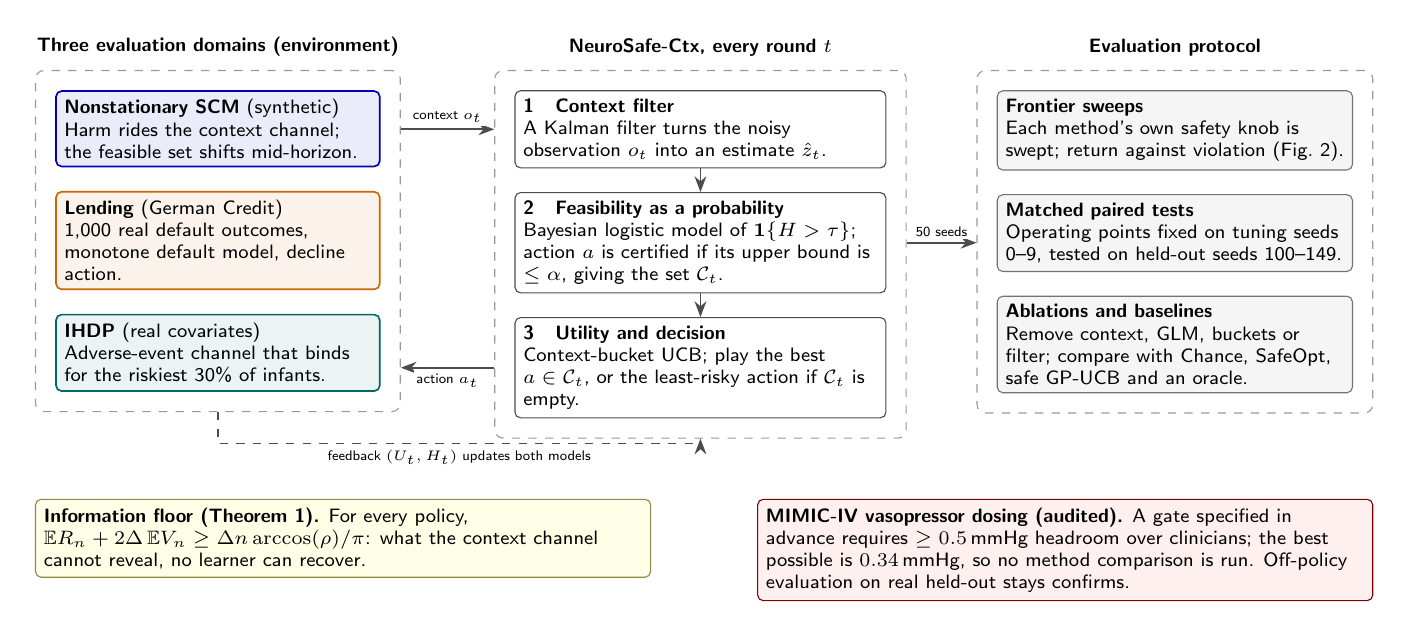
\begin{tikzpicture}[
  font=\sffamily\scriptsize, node distance=3mm and 6mm, >={Stealth[length=2mm]},
  dom/.style={draw=#1, fill=#1!8, rounded corners=2pt, text width=3.9cm, align=flush left, inner sep=3pt, line width=0.6pt},
  stp/.style={draw=black!70, fill=white, rounded corners=2pt, text width=4.5cm, align=flush left, inner sep=3pt},
  ev/.style={draw=black!55, fill=black!4, rounded corners=2pt, text width=4.3cm, align=flush left, inner sep=3pt},
  hdr/.style={font=\sffamily\scriptsize\bfseries, align=center},
  lab/.style={font=\sffamily\tiny, fill=white, inner sep=1pt},
  flow/.style={->, line width=0.6pt, draw=black!70}]
% ---------- column 1: domains (the environment)
\node[dom=blue!70!black] (scm) {\textbf{Nonstationary SCM} (synthetic)\\ Harm rides the context channel; the feasible set shifts mid-horizon.};
\node[dom=orange!80!black, below=of scm] (lend) {\textbf{Lending} (German Credit)\\ 1{,}000 real default outcomes, monotone default model, decline action.};
\node[dom=teal!80!black, below=of lend] (ihdp) {\textbf{IHDP} (real covariates)\\ Adverse-event channel that binds for the riskiest 30\% of infants.};
\begin{scope}[on background layer]
\node[draw=black!40, dashed, rounded corners=3pt, fit=(scm)(lend)(ihdp), inner sep=2.5mm] (env) {};
\end{scope}
\node[hdr, above=0.5mm of env] {Three evaluation domains (environment)};
% ---------- column 2: the decision rule
\node[stp, right=17mm of scm.north east, anchor=north west] (kf) {\textbf{1\quad Context filter}\\ A Kalman filter turns the noisy observation $o_t$ into an estimate $\hat z_t$.};
\node[stp, below=of kf] (glm) {\textbf{2\quad Feasibility as a probability}\\ Bayesian logistic model of $\mathbf 1\{H>\tau\}$; action $a$ is certified if its upper bound is $\le\alpha$, giving the set $\mathcal C_t$.};
\node[stp, below=of glm] (ucb) {\textbf{3\quad Utility and decision}\\ Context-bucket UCB; play the best $a\in\mathcal C_t$, or the least-risky action if $\mathcal C_t$ is empty.};
\begin{scope}[on background layer]
\node[draw=black!40, dashed, rounded corners=3pt, fit=(kf)(glm)(ucb), inner sep=2.5mm] (agent) {};
\end{scope}
\node[hdr, above=0.5mm of agent] {NeuroSafe-Ctx, every round $t$};
\draw[flow] (kf) -- (glm); \draw[flow] (glm) -- (ucb);
\draw[flow] (env.east |- kf.west) -- node[lab, above=1pt] {context $o_t$} (agent.west |- kf.west);
\draw[flow] (agent.west |- ucb.west) -- node[lab, below=1pt] {action $a_t$} (env.east |- ucb.west);
\draw[flow, dashed] (env.south) -- ++(0,-4mm) -| node[lab, pos=0.25, below=1pt] {feedback $(U_t,H_t)$ updates both models} (agent.south);
% ---------- column 3: evaluation
\node[ev, right=14mm of kf.north east, anchor=north west] (sweep) {\textbf{Frontier sweeps}\\ Each method's own safety knob is swept; return against violation (Fig.~2).};
\node[ev, below=of sweep] (match) {\textbf{Matched paired tests}\\ Operating points fixed on tuning seeds 0--9, tested on held-out seeds 100--149.};
\node[ev, below=of match] (abl) {\textbf{Ablations and baselines}\\ Remove context, GLM, buckets or filter; compare with Chance, SafeOpt, safe GP-UCB and an oracle.};
\begin{scope}[on background layer]
\node[draw=black!40, dashed, rounded corners=3pt, fit=(sweep)(match)(abl), inner sep=2.5mm] (evalbox) {};
\end{scope}
\node[hdr, above=0.5mm of evalbox] {Evaluation protocol};
\draw[flow] (agent.east |- glm.east) -- node[lab, above=1pt] {50 seeds} (evalbox.west |- glm.east);
% ---------- bottom band: theory and clinical audit
\coordinate (bandtop) at ($(env.south west)+(0,-11mm)$);
\node[ev, fill=yellow!10, draw=yellow!50!black, text width=7.6cm, anchor=north west] (thm) at (bandtop)
  {\textbf{Information floor (Theorem 1).} For every policy, $\mathbb E R_n+2\Delta\,\mathbb E V_n\ge\Delta n\arccos(\rho)/\pi$: what the context channel cannot reveal, no learner can recover.};
\node[ev, fill=red!6, draw=red!50!black, text width=7.6cm, anchor=north east] (mimic) at (bandtop -| evalbox.east)
  {\textbf{MIMIC-IV vasopressor dosing (audited).} A gate specified in advance requires $\ge0.5$\,mmHg headroom over clinicians; the best possible is $0.34$\,mmHg, so no method comparison is run. Off-policy evaluation on real held-out stays confirms.};
\end{tikzpicture}
}
\caption{\textbf{Overview of the study.} Three evaluation domains (left) emit a noisy context; at
every round NeuroSafe-Ctx filters it, certifies actions whose upper bound on the harm probability is
within the budget, and plays the most promising certified action or, if none is certified, the
least-risky one (centre). Methods are compared by frontier sweeps, by paired tests at operating points
fixed on tuning seeds, and by ablations (right). The information floor bounds every policy, and the
MIMIC-IV domain is audited by a gate fixed in advance (bottom).}
\label{fig:overview}
\end{figure}

\subsection*{Domains}
We use three domains for method comparison. (i) A nonstationary structural causal model (SCM) whose
harm rides a context channel and whose action--risk gain jumps mid-horizon, so that the feasible set
moves (shift 0.35, observation noise 0.15, $\tau=0.2$). (ii) German Credit lending~\cite{hofmann1994}
with the fixes described in the Results: the agent chooses a loan size or declines; harm is the
default probability of a monotone gradient-boosted model fitted to 1,000 real outcomes; utility is
loan size; the agent sees a noisy one-dimensional summary of the applicant ($\tau=0.25$). (iii)
IHDP~\cite{hill2011}: real covariates and fitted response surfaces, with an explicit adverse-event
channel that binds for the riskiest 30\% of infants, replacing an inert rank-based harm ($\tau=0.5$). This harm channel is constructed, because IHDP records no adverse events, and context matters in it by design, so we treat IHDP as a test of the mechanism rather than of real-world benefit. Response surfaces are fitted on the training split of the first realisation of the 100-realisation IHDP benchmark of Shalit et al.~\cite{shalit2017}, and each round draws an infant uniformly from the 75 infants of that realisation's test split; seeds vary the draws and noise, not the realisation.
A fourth, clinical domain built from MIMIC-IV is audited separately, as described below.

\subsection*{Baselines}
Chance is a context-blind chance-constrained rule that plays
$\arg\max_{a:\hat p(a)\le\alpha}\{\hat\mu_U(a)+\beta\hat\sigma_U(a)\}$, which is equation~(\ref{eq:obj})
under its own estimates. Reference SafeOpt~\cite{sui2015safeopt} is run contextually through the
\texttt{safeopt} package (version 0.16, with 15 lines of compatibility fixes for Python $\ge$3.10 and
NumPy $\ge$1.24 and no algorithmic change), with $a=0$ as its safe seed; it uses the package's contextual mode, in which separate Gaussian processes model utility and $-H$ with a squared-exponential kernel over action and context (automatic relevance determination), the context (scaled by its standard deviation on a separate environment seed) is held fixed during acquisition, an action is safe if its upper confidence bound on harm is at most $\tau$, and the safe seed is played when no action is safe in the current context; its action lengthscale and utility noise were tuned over $3\times2$ values on the tuning seeds. Safe GP-UCB is our own
reimplementation in the same style~\cite{sui2015safeopt,sui2018stageopt}; it certifies actions whose
Gaussian-process upper bound on harm is at most $\tau$ and plays GP-UCB utility among them. It explores
more aggressively than reference SafeOpt and the two are not equivalent, so we report both. Safe UCB-GLM, added in revision, follows the design of Amani et al.~\cite{amani2020glm}: a ridge-regularised logistic model of the harm event with frequentist confidence sets from the design matrix, a ridge-regression UCB for utility, the raw context and no forgetting, on the same features, warm-up and $\alpha$ grid as our method, with its two confidence multipliers tuned over nine values on the tuning seeds. We also
include a conservative linear UCB~\cite{kazerouni2017conservative} with the safest action as reference, which enforces a different notion of safety (cumulative reward relative to a baseline policy) and ignores harm, so it serves as a reference for that notion rather than as a competitor; an unconstrained UCB; NeuroSafe-CBO at its default setting and, in lending and
IHDP, an oracle that sees the true context.

\subsection*{Protocol and statistical analysis}
The horizon is 200 rounds. Hyperparameters were chosen on seeds 0--9, and every reported number is
from 50 held-out seeds, 100--149. Each method's own safety knob is swept: $\alpha$ for NeuroSafe-Ctx
and Chance, the confidence multiplier $\beta$ for safe GP-UCB and reference SafeOpt, and the budget for
the conservative bandit. For paired comparisons at matched operating points, our $\alpha$ is chosen on
the tuning seeds as the largest value whose violation rate does not exceed the baseline's; the
comparison is then run on the held-out seeds, so no pairing is chosen after seeing held-out results. The matching key is therefore realised violation, not nominal $\alpha$: when a baseline's realised violation exceeds its nominal level, the matched configuration of our method has a larger nominal $\alpha$ and a realised violation no higher than the baseline's.
For each comparison we report the mean paired difference over the 50 held-out seeds and a two-sided
95\% percentile bootstrap confidence interval (CI), resampling seeds; we describe a difference as
clear when its CI excludes zero. We report more than 100 such intervals and do not adjust them for
multiplicity, so we treat individual intervals as descriptive and base conclusions on frontier-level
patterns: for each baseline we interpolate our frontier at the baseline's operating points within our
violation range and count the points at which ours is higher. Figures show means with 95\% intervals
($1.96$ standard errors of the mean, $n=50$).

\subsection*{Ablation study}
To test which components matter, we remove one at a time while keeping everything else fixed and
sweeping the same $\alpha$ grid: no GLM (harm estimated per cell and passed through a Gaussian
cumulative distribution function, as in NeuroSafe-CBO), no context ($z\equiv0$), no bucketed
utility (a single bucket), and no filter (the raw channel). Each variant is compared with the full
method on its frontier and at $\alpha=0.15$. On IHDP we added, after the main runs, a calibrated
Beta--Bernoulli cell model with the same cells and shrinkage and an upper posterior quantile matching
the GLM's bound, to separate the effect of calibration from that of the GLM; its comparison with the
full method at equal $\alpha$ was specified before it was run, and a comparison at matched violation
was added afterwards and is labelled post hoc.

\subsection*{Clinical audit on MIMIC-IV}
The cohort comprises adult ICU stays with sepsis identified by ICD-9 or ICD-10 diagnosis codes, divided
into four-hour windows; we keep windows in which the mean arterial pressure (MAP) in the preceding
window was below 70\,mmHg and the patient was already receiving norepinephrine. This yields 65,100
windows from 6,197 stays. The action is one of five norepinephrine dose bins, utility is the next
window's MAP, and harm is a new arrhythmia. Stays were split in half; one half fits the simulator, and
the other (31,383 windows, 3,099 stays) is used only for evaluation. Three harm and three MAP model classes were compared by grouped 5-fold cross-validation on the fit half, with stays never split across folds (Supplementary Table~S4). Before running any agent we specified a gate, recorded in the analysis code before it was evaluated but not publicly registered: the domain is used for method comparison only if, at some $\alpha$, at least 80\%
of states have two or more safe doses, the MAP-maximising dose is unsafe in at least 10\% of states,
and the best constrained policy improves on clinicians by at least 0.5\,mmHg. The gate was evaluated on 8,000 windows sampled from the fit half. Because the simulator is fitted to that half, this choice favours passing the gate, so a failure there is conservative for a negative conclusion. On the held-out half the gate fails in the same way at every $\alpha$: the best constrained policy improves on clinicians by $0.21$\,mmHg at $\alpha=0.02$ and by at most $0.34$\,mmHg at any $\alpha$, equal to the unconstrained optimum. The real-data confirmation evaluates the $\alpha=0.02$
policy, softened to play its chosen dose with probability $1-\varepsilon$ ($\varepsilon=0.05$), against
clinicians on the held-out stays with weighted importance sampling~\cite{precup2000}, a fitted
behaviour-policy model, importance weights capped at 20, and a doubly robust
estimator~\cite{dudik2011,jiang2016}. An estimate is treated as reliable only if its effective sample
size~\cite{kong1992} is at least 200 and at least 1\% of decisions. Confidence intervals resample stays
(2,000 bootstrap replicates). An exploratory comparison of arrhythmia rates, which is not part of the gate, is reported in Supplementary Note~3.

\subsection*{Ethics statement}
This study used the MIMIC-IV database (version \verify{X.X})~\cite{johnson2023mimic}, accessed through
PhysioNet~\cite{goldberger2000} under its credentialed-access data use agreement after completion of
the required training. MIMIC-IV contains de-identified records; the collection of patient information and creation of the research resource was reviewed by the Institutional Review Board at the Beth Israel Deaconess Medical Center, which granted a waiver of informed consent and approved the data sharing initiative. All methods were performed in
accordance with the relevant guidelines and regulations. Patient-level data never left the
credentialed environment, and only aggregate statistics are reported or released. All MIMIC-IV processing was run locally under the data use agreement of the credentialed author (S.M.H.); no MIMIC-IV records or patient-level values were sent to any AI service, and AI assistants saw only analysis code and aggregate outputs of the kind reported in this paper, in line with PhysioNet's guidance on using MIMIC data with online services~\cite{physionet2025llm}.\verify{}

\subsection*{Software, reproducibility and use of AI tools}
All results were generated in a single recorded environment (Python 3.11.9, NumPy 1.26.4,
scikit-learn 1.9.1, SciPy 1.12.0, pandas 3.0.6; exact versions in \texttt{requirements-lock.txt}). Every
table and figure is generated programmatically from the released result files, and the code
repository (Code availability) contains a script for each step, listed in Supplementary Note~1. Regenerating every result in a second computing environment reproduced the SCM and IHDP results up to floating-point drift and changed no conclusion; on lending the fitted default model differs between library environments, so 4 of 42 single-$\alpha$ conclusions change category (none reverses) and we state lending results at the frontier level (Supplementary Note~2). AI
assistants were used extensively in this project: to write and debug code (including the method
implementation, baselines and environment fixes), to run experiments, to generate tables and figures
from result files, and to draft text. Theorem~\ref{thm:floor} and its proof were produced with AI
assistance. The authors are responsible for verifying every claim, proof step and number.

\section*{Results}

\subsection*{Our earlier method could not differ from its baseline}
Chance already implements equation~(\ref{eq:obj}) under its own estimates, and NeuroSafe-CBO may
replace Chance's pick only with an action at least as safe and $\varepsilon$ better in a context-mixed
utility estimate. Over 9,500 post-warm-up decisions on the held-out SCM, the pool of permitted
replacements was non-empty on 0.44\% of decisions, and on held-out seeds the two agents' returns (1.670
and 1.695) and violation rates (0.048 and 0.049) coincide; no number of seeds can separate agents that
act identically on 99.6\% of decisions. The context module also carried almost no context: under a
single declared protocol (decoupled SCM, 30 seeds of 400 steps, uniform actions, absolute Pearson
correlation with the latent confounder) the raw context observation scores 0.930, the published
predictive-coding latent 0.013, and a Kalman filter 0.929, so the deficit was in the implementation,
not the premise. Finally, the published update fitted the utility and harm models at both $(a,z_t)$
and $(a,0)$ with the same target, which teaches $f(a,z)=f(a,0)$, that is, to ignore context. For any
method defined as an improvement operator over a reference policy, the operator's activation rate
therefore belongs in the results table.

\subsection*{Four defects in the evaluation environments} The same discipline applied to the environments we had built or adapted to evaluate NeuroSafe-CBO found four defects in three environments (Table~\ref{tab:audit}).
Three of them invalidate safety comparisons without producing any visible error: numbers are computed,
confidence intervals are tight, and the conclusions are wrong. We fixed the two lending defects,
replaced the inert IHDP harm, and removed the original MIMIC-IV formulation, in which observational
acuity data could not produce a tension between safety and utility; the MIMIC-IV domain audited below
is a separate vasopressor-dosing formulation built for this study. We recommend that safe-decision
benchmarks report the oracle's violation rate, the fraction of contexts with an empty feasible set,
and the performance of an unconstrained agent alongside every result.

\begin{table}[t]
\caption{\textbf{Environment defects, how each was measured, and what we did.} ``Violation'' is the
realised rate against $\alpha=0.15$.}
\label{tab:audit}
\centering\small
\begin{tabular}{p{2.3cm}p{6.0cm}p{6.4cm}}
\toprule
Environment & Defect (measured) & Consequence and action \\
\midrule
Lending (German Credit) & An unconstrained tree ensemble gave mean $P(\text{default})$ of
$0.25\to0.20\to0.41\to0.22$ as loan size rose: larger loans ``lowered'' risk on half the grid. &
No coherent feasible set to learn. \textbf{Fixed}: monotone constraints (risk non-decreasing in loan
size and risk score); in-sample AUC on real defaults $0.814$. \\
Lending & No decline action: for 40\% of applicants every action was a loan above the risk limit. &
Realised violation $0.36$ for both evaluated agents in the original results. \textbf{Fixed}: $a=0$
declines (no loan, no profit, no exposure). \\
IHDP & Harm was the within-arm rank of the outcome, uniform on $[0,1]$ by construction, so
$\mathbb P(H>0.5)\approx0.5$ for \emph{any} policy. & All agents violated at $0.489$--$0.490$; the
safety axis could not separate methods. \textbf{Replaced} by an explicit adverse-event channel that
binds for the riskiest 30\%. \\
MIMIC-IV (original formulation) & Action = admission type ordered by \emph{observed mortality};
utility $5(1-a)$. Both favour $a=0$. & An unconstrained agent scored $4.57$ return at $0.009$ violation
against $3.24$ at $0.063$ for Chance. \textbf{Removed}: observational acuity data cannot produce a
safety--utility tension. \\
\bottomrule
\end{tabular}
\end{table}

\subsection*{The information floor is attained}
Beyond the proof, \texttt{experiments/verify\_theorem.py} checks the pathwise identity, Sheppard's formula (maximum error $0.0014$ over 20 values of $\rho$) and Corollary~\ref{cor:gauss} against seven policy families, including randomised and feedback-adaptive ones; none falls below the floor. On the simulated
Gaussian instance (Supplementary Table~S6; Supplementary Fig.~S1) the Bayes rule matches
$\arccos(\rho)/\pi$ at every $\rho$ (largest discrepancy $0.004$). The per-decision
$\alpha$-constrained Bayes rule keeps violations near $0.01$ and pays $0.18$--$0.47$, and our method,
learning online for 600 rounds, keeps violations at $0.008$--$0.060$ but reaches $0.41$--$0.50$: it is
correctly safe but substantially more conservative than the constrained optimum at this horizon. Pricing violations at the budget's own rate, $\lambda=\Delta/0.15$ (Proposition~\ref{prop:alpha}), the $\alpha$-constrained Bayes rule meets the weighted floor to within the rounding of Supplementary Table~S6 (0.227 against 0.230 at $\rho=0.928$, 0.353 against 0.357 at $0.812$, 0.422 against 0.425 at $0.707$, and 0.489 against 0.490 at $0.5$). At that price the online learner beats always declining (0.501) only when the channel is informative ($\rho\ge0.812$); at $\rho\le0.707$ even the optimal rule is within 15\% of always declining, so there is little to gain, and the learner's exploration costs more than it earns.



\subsection*{Frontiers across the three domains}
Figure~\ref{fig:domains} shows every method's safety--utility frontier on the three domains.  Full matched comparisons for the SCM and lending are in Supplementary Tables~S1 and S2.

\begin{figure}[t]
\centering
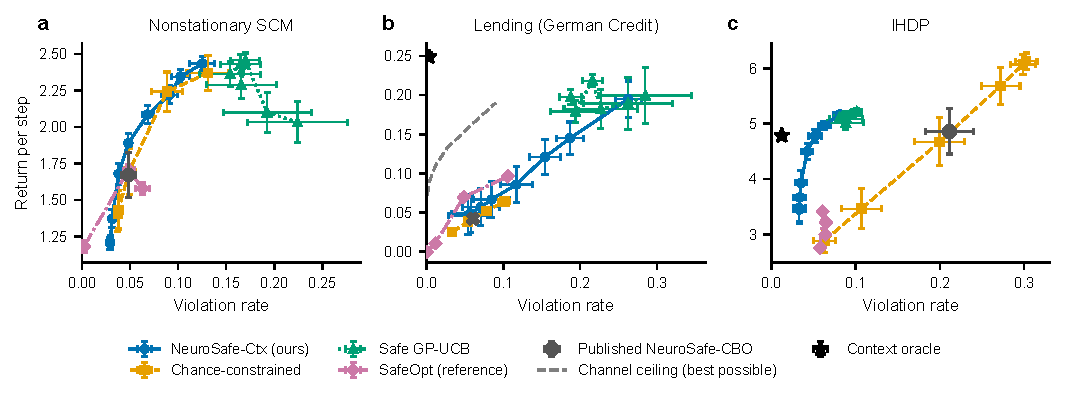
\includegraphics[width=\linewidth]{figures/fig_domains.pdf}
\caption{\textbf{Safety--utility frontiers on 50 held-out seeds.} \textbf{a}, Nonstationary SCM.
\textbf{b}, Lending with real default labels; the dashed line is the best return any agent seeing
only the context channel can achieve (channel ceiling). \textbf{c}, IHDP with a binding harm channel.
Each point is one setting of a method's safety knob; bars are 95\% intervals ($1.96$ standard errors
of the mean, $n=50$ seeds). Up and to the left is better. The conservative bandit and the
unconstrained UCB lie outside the plotted range or above the budget (violation $0.65$--$0.75$ on the
SCM, $0.87$--$0.89$ on lending and $0.31$ on IHDP for the conservative bandit; $0.33$, $0.95$ and $0.31$
for the unconstrained UCB) and are omitted.}
\label{fig:domains}
\end{figure}

\subsection*{IHDP: improving both axes at once}
Against Chance, NeuroSafe-Ctx improves both axes at Chance's two most conservative settings: $+1.615$
return (95\% CI $+1.405$ to $+1.799$) with $-0.021$ violation ($-0.035$ to $-0.007$), and $+1.703$ with
$-0.026$, all four intervals excluding zero (Table~\ref{tab:m-ihdp}). These comparisons are matched on realised violation measured on tuning seeds: the headline pairs our $\alpha=0.15$ with Chance's $\alpha=0.02$ because Chance's realised violation at $\alpha=0.02$ is already $0.063$, above our $0.043$ at $\alpha=0.15$. Two features of the frontiers qualify them. First, Chance's
realised violation is roughly two to three times its nominal level ($0.063$ at $\alpha=0.02$, $0.107$
at $0.05$, $0.200$ at $0.10$) and never falls below $0.063$, so below that level the comparison is one
of reachability rather than of return at equal violation. Second, NeuroSafe-Ctx finds no certified
action on 78--94\% of decisions at $\alpha\le0.05$ (17\% at $\alpha=0.15$) and then plays its
lowest-certified-harm action; its violation does not fall below $0.033$, so for $\alpha\le0.03$ it exceeds the nominal level (see Limitations). 

\subsection*{IHDP: comparison with SafeOpt-style baselines}
Against reference SafeOpt the margin is larger: $+1.36$ to $+2.02$ return at all four of its settings,
with lower violation at three (CIs excluding zero) and equal violation at the fourth, and our frontier
is above it at all four comparable points. Against our own safe GP-UCB the result is a trade: that
baseline earns $5.02$--$5.22$ against our $4.78$--$5.17$, more at four of six settings (CIs excluding
zero), while our violation is lower at all six. NeuroSafe-CBO reaches $4.86$ at violation $0.211$, and the context-observing oracle $4.79$ at $0.013$. Against Safe UCB-GLM, the closest prior design, our frontier is higher at both comparable points ($+0.14$ and $+0.12$); at equal $\alpha$ ours earns more for $\alpha\le0.05$ ($+0.92$ at $\alpha=0.02$) and violates less for $\alpha\ge0.15$ (by $0.022$--$0.060$) (Supplementary Table~S10).

\begin{table}[t]
\caption{\textbf{Paired tests at operating points matched on tuning seeds, IHDP with a binding harm
channel.} Differences are ours minus the baseline over 50 held-out seeds, with 95\% bootstrap CIs; bold
marks CIs that exclude zero.}
\label{tab:m-ihdp}
\centering\small
\resizebox{\linewidth}{!}{\begin{tabular}{lcllll}
\toprule
Baseline @knob & our $\alpha$ & Return (base$\to$ours) & $\Delta$R [95\% CI] & Violation (base$\to$ours) & $\Delta$V [95\% CI] \\
\midrule
Chance @0.02 & 0.15 & 2.885$\to$4.500 & \textbf{+1.615} [+1.405, +1.799] & 0.0632$\to$0.0427 & \textbf{-0.0205} [-0.0355, -0.0070] \\
Chance @0.05 & 0.35 & 3.466$\to$5.168 & \textbf{+1.703} [+1.326, +2.045] & 0.1072$\to$0.0814 & \textbf{-0.0258} [-0.0504, -0.0041] \\
Chance @0.1 & 0.35 & 4.675$\to$5.168 & \textbf{+0.494} [+0.080, +0.914] & 0.1997$\to$0.0814 & \textbf{-0.1183} [-0.1467, -0.0905] \\
Chance @0.15 & 0.35 & 5.682$\to$5.168 & \textbf{-0.514} [-0.819, -0.174] & 0.2720$\to$0.0814 & \textbf{-0.1906} [-0.2127, -0.1664] \\
Chance @0.25 & 0.35 & 6.070$\to$5.168 & \textbf{-0.901} [-1.050, -0.706] & 0.2987$\to$0.0814 & \textbf{-0.2173} [-0.2303, -0.2016] \\
Chance @0.35 & 0.35 & 6.130$\to$5.168 & \textbf{-0.962} [-1.067, -0.814] & 0.3025$\to$0.0814 & \textbf{-0.2211} [-0.2322, -0.2076] \\
Safe GP-UCB @0.5 & 0.35 & 5.218$\to$5.168 & \textbf{-0.049} [-0.101, -0.003] & 0.1013$\to$0.0814 & \textbf{-0.0199} [-0.0246, -0.0150] \\
Safe GP-UCB @1 & 0.35 & 5.177$\to$5.168 & -0.009 [-0.065, +0.040] & 0.0941$\to$0.0814 & \textbf{-0.0127} [-0.0168, -0.0087] \\
Safe GP-UCB @1.5 & 0.25 & 5.136$\to$4.970 & \textbf{-0.166} [-0.225, -0.113] & 0.0847$\to$0.0626 & \textbf{-0.0221} [-0.0263, -0.0174] \\
Safe GP-UCB @2 & 0.25 & 5.116$\to$4.970 & \textbf{-0.146} [-0.210, -0.087] & 0.0809$\to$0.0626 & \textbf{-0.0183} [-0.0233, -0.0131] \\
Safe GP-UCB @3 & 0.2 & 5.092$\to$4.777 & \textbf{-0.314} [-0.473, -0.189] & 0.0891$\to$0.0520 & \textbf{-0.0371} [-0.0582, -0.0200] \\
Safe GP-UCB @4 & 0.25 & 5.018$\to$4.970 & -0.048 [-0.168, +0.056] & 0.0884$\to$0.0626 & \textbf{-0.0258} [-0.0489, -0.0077] \\
SafeOpt (reference) @1 & 0.2 & 2.757$\to$4.777 & \textbf{+2.020} [+1.900, +2.123] & 0.0581$\to$0.0520 & -0.0061 [-0.0135, +0.0036] \\
SafeOpt (reference) @2 & 0.2 & 2.998$\to$4.777 & \textbf{+1.779} [+1.651, +1.887] & 0.0642$\to$0.0520 & \textbf{-0.0122} [-0.0187, -0.0038] \\
SafeOpt (reference) @3 & 0.2 & 3.214$\to$4.777 & \textbf{+1.563} [+1.440, +1.668] & 0.0649$\to$0.0520 & \textbf{-0.0129} [-0.0189, -0.0051] \\
SafeOpt (reference) @4 & 0.2 & 3.417$\to$4.777 & \textbf{+1.361} [+1.238, +1.469] & 0.0610$\to$0.0520 & \textbf{-0.0090} [-0.0144, -0.0018] \\
\bottomrule
\end{tabular}
}
\end{table}

\subsection*{IHDP: the advantage tracks what the context reveals}
Because the IHDP harm channel is constructed, we tested in revision whether the gain comes from the mechanism or the construction, adding observation noise so that the correlation $\rho$ between the observed context and the signal that drives harm falls from $0.99$ (the setting above) to $0.3$, holding everything else fixed (Supplementary Table~S8). The advantage falls as our claim predicts: the mean gain of our frontier over Chance at comparable violation is $+2.09$ at $\rho=0.99$, $+1.38$ at $0.9$, $+0.60$ at $0.7$ and $+0.13$ at $0.3$. The safety advantage of the headline pair vanishes for $\rho\le0.95$ and reverses for $\rho\le0.7$ ($\Delta V=+0.032$, CI $+0.012$ to $+0.057$, at $\rho=0.3$), and our lowest reachable violation rises from $0.033$ to $0.083$. Chance, which ignores context, is unaffected.

\subsection*{Nonstationary SCM: gains only where safety is tight}
Against Chance, the gain is concentrated where safety is tight: at Chance's three most conservative
settings NeuroSafe-Ctx improves return by $+0.245$ to $+0.272$ at unchanged violation ($\approx0.038$).
At Chance's default ($\alpha=0.15$) it has equal return and lower violation ($0.038$ against $0.049$,
CI excluding zero); at Chance's two loosest settings the matched point is a trade, with lower return
and lower violation, and on the frontier the two curves meet; interpolating our frontier at Chance's
points, ours is higher at 4 of 5 comparable points. Safe GP-UCB never falls below violation $0.154$;
at $\alpha=0.35$ (violation $0.125$) our method has lower violation than every GP-UCB setting and higher
or equal return at all six. Reference SafeOpt operates at violation $0.002$--$0.063$; our frontier is
above it at both comparable points, by $+0.19$ and $+0.45$, and at its two most conservative settings it
collapses onto its safe seed (return $1.182$ at violation $0.002$), as its design prescribes when the
safe set cannot be expanded. Against Safe UCB-GLM our method earns more and violates less at every $\alpha\ge0.05$ (CIs excluding zero), and its frontier is higher at all five comparable points (Supplementary Table~S10). The conservative bandit ignores harm and violates at $0.65$--$0.75$, and
the unconstrained UCB reaches $2.352$ return at $0.332$ violation.

\subsection*{Lending: no advantage on real default labels}
Against Chance, no matched-point difference excludes zero on either axis (Supplementary Table~S2).
On the frontier ours is higher at all 4 comparable points, but by only $0.008$--$0.013$: in practical
terms, a tie. Safe GP-UCB is better where both operate: at its three least conservative settings
(violation $0.19$--$0.22$) it earns $0.179$--$0.218$ against our $0.145$ at $0.187$, more at all three
(CIs excluding zero), and it is above our frontier at 4 of 5 comparable points, although our method and
Chance also operate at violation $0.03$--$0.12$, a region GP-UCB never reaches (its minimum is $0.188$).
Reference SafeOpt is at least as good as our method: neither matched return difference excludes zero ($-0.021$, CI $-0.040$ to $+0.005$, at its $\beta=2$ point; $-0.010$, CI $-0.029$ to $+0.014$, at $\beta=1$), and its frontier lies above ours at the one comparable point. Which method is
preferable on lending therefore depends on the risk budget, and we claim no advantage there.

\subsection*{Lending: most of the gap to the oracle is missing information}
Every learner is far from the oracle ($0.249$ at violation $0.003$), which sees both applicant covariates where agents see only their noisy average. The best policy available from that channel (dashed line in Fig.~\ref{fig:domains}b) earns $0.090$ at violation $0.004$, only 36\% of the oracle's return, so most of the gap is missing information, the regime Theorem~\ref{thm:floor} describes; but at violation $\approx0.05$ the channel allows $0.154$ while every learner, ours included, earns $0.038$--$0.046$, so learning also falls short.

\begin{table}[t]
\caption{\textbf{Ablations on held-out seeds.} ``Frontier'': at how many of the variant's operating
points (within our violation range) the full method's interpolated return is higher, and the range of
the difference. ``$\alpha=0.15$'': full method minus variant; positive $\Delta$R favours the full
method, and positive $\Delta$V means the full method violates more. Bold: CI excludes zero.}
\label{tab:abl}
\centering
\resizebox{\linewidth}{!}{\begin{tabular}{lllllll}
\toprule
 & \multicolumn{2}{c}{SCM} & \multicolumn{2}{c}{Lending} & \multicolumn{2}{c}{IHDP} \\
\cmidrule(lr){2-3}\cmidrule(lr){4-5}\cmidrule(lr){6-7}
Variant & frontier: full above & $\alpha{=}0.15$: $\Delta$R / $\Delta$V & frontier: full above & $\alpha{=}0.15$: $\Delta$R / $\Delta$V & frontier: full above & $\alpha{=}0.15$: $\Delta$R / $\Delta$V \\
\midrule
no GLM (Gaussian-CDF cells) & 8/9 (-0.006..+0.142) & +0.078 / +0.0022 & 1/3 (-0.017..+0.005) & \textbf{+0.046} / \textbf{+0.0650} & 8/8 (+0.264..+1.697) & +0.112 / \textbf{-0.0185} \\
no context ($z\equiv0$) & 4/6 (-0.043..+0.067) & \textbf{-0.095} / \textbf{-0.0088} & 8/8 (+0.006..+0.076) & +0.019 / -0.0172 & none (min $V$ 0.126) & \textbf{+0.609} / \textbf{-0.0981} \\
no bucketed utility & 3/9 (-0.079..+0.016) & +0.009 / \textbf{+0.0069} & 1/8 (-0.000..+0.001) & +0.001 / +0.0002 & 6/9 (-0.053..+0.104) & +0.011 / +0.0007 \\
no filter (raw channel) & 4/9 (-0.019..+0.017) & -0.014 / -0.0024 & 3/9 (-0.002..+0.001) & +0.000 / +0.0001 & 1/5 (-0.009..+0.002) & +0.004 / +0.0001 \\
\bottomrule
\end{tabular}
}
\end{table}

\subsection*{Ablation: context matters most, and mainly for safety}
Table~\ref{tab:abl} shows that two of the four components are unnecessary. Context-conditional feasibility matters most on IHDP, and there mainly for safety: at
$\alpha=0.15$ the full method has higher return ($+0.609$, CI $+0.187$ to $+1.008$) and lower violation
($-0.098$, CI $-0.133$ to $-0.066$), and the two frontiers do not overlap, because the context-free
variant's lowest violation ($0.126$) exceeds the full method's highest ($0.081$). This holds even though
that variant defers to its least-risky action whenever nothing is certified, because without context
that action is the same for every infant. On lending, removing context lowers the frontier at all 8
comparable points (by $0.006$--$0.076$), although the $\alpha=0.15$ difference does not exclude zero;
on the SCM its effect is mixed, and at $\alpha=0.15$ the context-free variant has higher return and
higher violation.

\subsection*{Ablation: the harm model matters for different reasons}
On the SCM, without the GLM violation cannot be pushed below $0.056$ at any $\alpha$, whereas the full
method reaches $0.029$, so the low-risk region is unreachable, and the full method is higher at 8 of 9
frontier points. On IHDP, where harm is a rare binary event, the ablation's Gaussian cells underestimate
violation probabilities: the variant almost never finds its feasible set empty, its realised violation
at $\alpha=0.02$ is $0.049$ (2.5 times nominal), and the full method is above it at all 8 comparable
frontier points (by $+0.26$ to $+1.70$). Part of this gap is calibration rather than the GLM itself:
the calibrated Beta--Bernoulli cell model is safer but far more conservative, and in the pre-specified
same-$\alpha$ comparison the full method has higher return at $\alpha\in\{0.10,0.15,0.20\}$ ($+1.38$
to $+2.06$) but also higher violation at $0.15$ and $0.20$ ($+0.012$ and $+0.019$), so it does not meet
our criterion for a win. A post hoc comparison at matched violation, possible at only two points,
favours the GLM ($+1.05$, CI $+0.41$ to $+1.39$, at $V\approx0.043$; $+0.31$, CI $+0.12$ to $+0.51$, at
$V\approx0.072$; Supplementary Table~S3). We read this as suggestive evidence that the GLM's advantage
on IHDP is data efficiency: sharing strength across contexts lets it certify higher-return actions
within 200 rounds. On lending the GLM trades violation for return: at $\alpha=0.15$ it raises both (by
$0.046$ and $0.065$), and the frontiers cross.

\subsection*{Ablation: bucketed utility and filter add nothing}
The bucketed utility and the Kalman filter show no consistent benefit in any domain (frontier differences within $\pm0.08$ on the SCM, $\pm0.002$ on lending and $-0.05$ to $+0.10$ on IHDP). For the filter this is expected: the raw channel already correlates $0.93$ with the context on the SCM, and lending and IHDP contexts are independent, where the filter reduces to the identity. We retain both only because they are harmless, and claim neither as a contribution.

\subsection*{MIMIC-IV: the gate fails}
The arrhythmia model's in-sample AUC of $0.806$ does not survive grouped cross-validation
($0.62$--$0.64$ across three model classes); the model selected by cross-validated log-loss reaches AUC
$0.632$, and the MAP model $R^2=0.266$, on held-out stays (Supplementary Table~S4). At $\alpha=0.02$
the constraint offers a real choice (83\% of states) and changes the MAP-maximising dose in 21\% of
states, at a cost of $0.59$\,mmHg when it does, but the best constrained policy improves on clinicians
by only $0.21$\,mmHg, and even the unconstrained optimum by $0.34$\,mmHg, an upper bound because it
maximises the model's own predictions (Supplementary Table~S7). The gate fails at every $\alpha$,
so we run no agent comparisons on MIMIC-IV and make no claim about our method there.



\subsection*{MIMIC-IV: real-data confirmation}
Off-policy evaluation of the $\alpha=0.02$ policy on held-out stays (effective sample size 20\% of
decisions) confirms the absence of headroom: $+0.046$\,mmHg, CI $-0.182$ to $+0.285$
(Table~\ref{tab:mimic-ope}); the doubly robust estimate, $+0.42$, is probably biased upward by its
outcome model and is also below the threshold. Because the simulator's harm model is weak (AUC $0.632$), the conclusion is scoped to this formulation and these covariates: no policy shows meaningful headroom here, which does not establish that context-conditional dosing cannot help. An exploratory comparison of arrhythmia rates, likely confounded by severity, is reported in Supplementary Note~3 and is not used for any conclusion.

\begin{table}[t]
\caption{\textbf{MIMIC-IV off-policy evaluation on held-out stays: constrained policy ($\alpha=0.02$)
against clinicians.} Intervals resample stays; DR is the doubly robust estimate. The arrhythmia row is exploratory and likely confounded by severity (Supplementary Note~3).}
\label{tab:mimic-ope}
\centering\small
\resizebox{\linewidth}{!}{\begin{tabular}{lcccc}
\toprule
Outcome & clinicians & constrained policy (WIS) & difference [95\% CI, stays resampled] & difference (DR) \\
\midrule
MAP (mmHg) & 66.82 & 66.87 & +0.046 [-0.182, +0.285] & +0.415 \\
arrhythmia rate & 0.0181 & 0.0131 & -0.0050 [-0.0078, -0.0019] & -0.0030 \\
\bottomrule
\end{tabular}
}
\end{table}



\section*{Limitations}

\subsection*{Scale and realism of the benchmarks}
The three method-comparison domains are small: one synthetic and two built on real covariates (1,000
lending outcomes; IHDP), each with a one-dimensional observed context and a horizon of 200 rounds. Real credit and clinical decisions use many covariates, arrive over months or years, and face
distribution shift that a single mid-horizon jump does not capture. Our conclusions are about the
mechanism---when context-conditional feasibility can help---and not about deployable performance.

\subsection*{Constructed and fitted harm channels}
The IHDP harm channel is constructed, because IHDP records no adverse events, and the lending harm is
the output of a fitted default model rather than observed defaults under the agent's own decisions.
The lending dose--response is estimated from observational records in which the lender chose amounts
partly on risk, so it is not a causal quantity; this does not affect the internal validity of
algorithm comparisons against the shared fitted environment, but it does limit external claims. The
monotone constraint is a modelling assumption justified by domain knowledge rather than by the data,
and lending's single-$\alpha$ effects are of the same order as the variation between computing
environments.

\subsection*{Statistical multiplicity and tuning budgets}
We report more than 100 confidence intervals without adjustment, so a few of them will exclude zero by
chance; we have therefore based conclusions on frontier-level patterns that hold across many operating
points. Our method was tuned over 18 configurations, reference SafeOpt originally over 6 and Safe UCB-GLM over 9. Re-tuning reference SafeOpt over 18 configurations, the same budget as ours, changes no conclusion: our frontier stays above it at all four comparable IHDP points (by $1.20$--$2.05$, against $1.52$--$2.13$ before) and both SCM points ($0.27$--$0.47$), and on lending the larger grid selects the same configuration (Supplementary Note~5).

\subsection*{How safety is achieved at small budgets}
At small $\alpha$ our method's safety comes largely from its fallback to the least-risky action (78--94\% of IHDP decisions at $\alpha\le0.05$), not from active optimisation. Its realised violation stays at or below the nominal level for every $\alpha\ge0.075$ in all three domains, but not below that. A decomposition added in revision locates the excess (Supplementary Table~S9). On the SCM it comes almost entirely from the ten random warm-up rounds ($0.027$ of $0.029$ at $\alpha=0.02$); a variant whose warm-up plays the safest action stays within budget at every $\alpha$ tested and also earns more ($1.75$ against $1.37$ at $\alpha=0.05$). On IHDP the safest action, no treatment, itself violates at $0.021$, so $\alpha\le0.02$ leaves no room to learn; the same variant meets the budget for $\alpha\ge0.03$ but earns much less ($2.39$ against $3.48$ at $\alpha=0.05$) because it rarely tries treatment. Every reported comparison uses the method as frozen on tuning seeds, and we claim calibrated behaviour only for $\alpha\ge0.075$.

\subsection*{Clinical validity of the MIMIC-IV audit}
A clinician would raise several objections to the MIMIC-IV domain, and we accept them. The simulator
discriminates harm only weakly on held-out patients (AUC $0.632$); the cohort is defined by diagnosis
codes rather than clinical sepsis criteria~\cite{singer2016}; MAP in the next four-hour window is a
surrogate, not a patient-centred outcome such as mortality or organ support; four-hour windows are
coarse relative to how vasopressors are titrated; and other vasopressors and fluids are treated only as
covariates. The exploratory harm finding is observational and may be confounded by severity. The audit
supports a negative conclusion about this formulation, not any recommendation about dosing.

\subsection*{Scope of the theory}
Theorem~\ref{thm:floor} is a lower bound on a stylised two-action class. We give no upper bound for our
method, which sits well above the constrained optimum at $n=600$ on that class, and we do not show how
far the floor transfers to multi-action, autocorrelated settings such as our SCM.

\section*{Conclusion}
A method that ties its baseline may be redundant with it by construction, and a benchmark that reports
tight confidence intervals may be measuring nothing; both are cheap to check. Once the method and its
benchmarks were repaired, context-conditional feasibility helped decisively where feasibility genuinely
depends on context (IHDP: better than a chance-constrained rule on both axes at once, and than reference
SafeOpt in return at equal or lower violation), helped where safety budgets are tight (the SCM), and did
not help on real lending data, where it ties the chance-constrained rule and is matched or beaten by
both SafeOpt-style baselines. On a real clinical domain, a gate fixed in advance showed that there was
nothing for any policy to gain over clinicians in blood pressure. Theorem~\ref{thm:floor} explains why
gains of this kind are bounded: the information in the context channel, not the learning algorithm,
sets a floor that every policy shares. Future work should test the mechanism with richer contexts and longer horizons, and derive an upper bound that matches the floor.

\medskip\noindent\textbf{Data availability.} The German Credit data are publicly available from the UCI Machine Learning Repository~\cite{hofmann1994}.
The IHDP covariates and response surfaces are publicly available~\cite{hill2011}. MIMIC-IV is available to
credentialed researchers through PhysioNet~\cite{johnson2023mimic,goldberger2000}; under its data use
agreement we cannot share patient-level data or data derived from them, but the aggregate statistics
reported here (\texttt{results/v3/mimic/audit.json}) and the code that produces them from the source
database are released. All other result files supporting the findings are available in the code
repository.

\medskip\noindent\textbf{Code availability.} All code, result files and scripts that regenerate every table and figure are available at \coderepo{} (archived release: \url{https://doi.org/10.5281/zenodo.23642195}). Supplementary Note~1 lists the commands in order.


{\footnotesize\setlength{\itemsep}{0pt}\setlength{\parskip}{0pt}
\begin{thebibliography}{99}
\bibitem{sui2015safeopt} Sui, Y., Gotovos, A., Burdick, J. \& Krause, A. Safe exploration for optimization with Gaussian processes. In \emph{Proc. 32nd International Conference on Machine Learning} 997--1005 (PMLR, 2015).
\bibitem{sui2018stageopt} Sui, Y., Zhuang, V., Burdick, J. \& Yue, Y. Stagewise safe Bayesian optimization with Gaussian processes. In \emph{Proc. 35th International Conference on Machine Learning} (PMLR, 2018).
\bibitem{berkenkamp2023} Berkenkamp, F., Krause, A. \& Schoellig, A. P. Bayesian optimization with safety constraints: safe and automatic parameter tuning in robotics. \emph{Mach. Learn.} \textbf{112}, 3713--3747 (2023).
\bibitem{wu2016conservative} Wu, Y., Shariff, R., Lattimore, T. \& Szepesv\'ari, C. Conservative bandits. In \emph{Proc. 33rd International Conference on Machine Learning} (PMLR, 2016).
\bibitem{kazerouni2017conservative} Kazerouni, A., Ghavamzadeh, M., Abbasi-Yadkori, Y. \& Van Roy, B. Conservative contextual linear bandits. In \emph{Advances in Neural Information Processing Systems 30} (2017).
\bibitem{amani2019linear} Amani, S., Alizadeh, M. \& Thrampoulidis, C. Linear stochastic bandits under safety constraints. In \emph{Advances in Neural Information Processing Systems 32} (2019).
\bibitem{pacchiano2021} Pacchiano, A., Ghavamzadeh, M., Bartlett, P. \& Jiang, H. Stochastic bandits with linear constraints. In \emph{Proc. 24th International Conference on Artificial Intelligence and Statistics} (PMLR, 2021).
\bibitem{altman1999cmdp} Altman, E. \emph{Constrained Markov Decision Processes} (Chapman \& Hall/CRC, 1999).
\bibitem{achiam2017cpo} Achiam, J., Held, D., Tamar, A. \& Abbeel, P. Constrained policy optimization. In \emph{Proc. 34th International Conference on Machine Learning} 22--31 (PMLR, 2017).
\bibitem{garcia2015survey} Garc\'ia, J. \& Fern\'andez, F. A comprehensive survey on safe reinforcement learning. \emph{J. Mach. Learn. Res.} \textbf{16}, 1437--1480 (2015).
\bibitem{charnes1959} Charnes, A. \& Cooper, W. W. Chance-constrained programming. \emph{Manage. Sci.} \textbf{6}, 73--79 (1959).
\bibitem{hill2011} Hill, J. L. Bayesian nonparametric modeling for causal inference. \emph{J. Comput. Graph. Stat.} \textbf{20}, 217--240 (2011).
\bibitem{shalit2017} Shalit, U., Johansson, F. D. \& Sontag, D. Estimating individual treatment effect: generalization bounds and algorithms. In \emph{Proc. 34th International Conference on Machine Learning} 3076--3085 (PMLR, 2017).
\bibitem{dorie2019} Dorie, V., Hill, J., Shalit, U., Scott, M. \& Cervone, D. Automated versus do-it-yourself methods for causal inference: lessons learned from a data analysis competition. \emph{Stat. Sci.} \textbf{34}, 43--68 (2019).
\bibitem{johnson2023mimic} Johnson, A. E. W. \emph{et al.} MIMIC-IV, a freely accessible electronic health record dataset. \emph{Sci. Data} \textbf{10}, 1 (2023).
\bibitem{komorowski2018} Komorowski, M., Celi, L. A., Badawi, O., Gordon, A. C. \& Faisal, A. A. The Artificial Intelligence Clinician learns optimal treatment strategies for sepsis in intensive care. \emph{Nat. Med.} \textbf{24}, 1716--1720 (2018).
\bibitem{henderson2018} Henderson, P. \emph{et al.} Deep reinforcement learning that matters. In \emph{Proc. 32nd AAAI Conference on Artificial Intelligence} (2018).
\bibitem{pineau2021} Pineau, J. \emph{et al.} Improving reproducibility in machine learning research. \emph{J. Mach. Learn. Res.} \textbf{22}, 1--20 (2021).
\bibitem{gundersen2018} Gundersen, O. E. \& Kjensmo, S. State of the art: reproducibility in artificial intelligence. In \emph{Proc. 32nd AAAI Conference on Artificial Intelligence} (2018).
\bibitem{neurosafecbo} Hasan, M. M. NeuroSafe-CBO: source code. \emph{GitHub} https://github.com/MahmudulHasanJoy/NeuroSafe-CBO \verify{(year; replace with the earlier paper or preprint if one exists)}.
\bibitem{amani2020glm} Amani, S., Alizadeh, M. \& Thrampoulidis, C. Generalized linear bandits with safety constraints. In \emph{Proc. IEEE International Conference on Acoustics, Speech and Signal Processing} (2020).
\bibitem{srinivas2010} Srinivas, N., Krause, A., Kakade, S. \& Seeger, M. Gaussian process optimization in the bandit setting: no regret and experimental design. In \emph{Proc. 27th International Conference on Machine Learning} 1015--1022 (2010).
\bibitem{rasmussen2006} Rasmussen, C. E. \& Williams, C. K. I. \emph{Gaussian Processes for Machine Learning} (MIT Press, 2006).
\bibitem{moradipari2021} Moradipari, A., Amani, S., Alizadeh, M. \& Thrampoulidis, C. Safe linear Thompson sampling with side information. \emph{IEEE Trans. Signal Process.} \textbf{69}, 3755--3767 (2021).
\bibitem{liu2021} Liu, X., Li, B., Shi, P. \& Ying, L. An efficient pessimistic-optimistic algorithm for stochastic linear bandits with general constraints. In \emph{Advances in Neural Information Processing Systems 34} (2021).
\bibitem{filippi2010} Filippi, S., Capp\'e, O., Garivier, A. \& Szepesv\'ari, C. Parametric bandits: the generalized linear case. In \emph{Advances in Neural Information Processing Systems 23} (2010).
\bibitem{li2017glm} Li, L., Lu, Y. \& Zhou, D. Provably optimal algorithms for generalized linear contextual bandits. In \emph{Proc. 34th International Conference on Machine Learning} (PMLR, 2017).
\bibitem{russac2021} Russac, Y., Faury, L., Capp\'e, O. \& Garivier, A. Self-concordant analysis of generalized linear bandits with forgetting. In \emph{Proc. 24th International Conference on Artificial Intelligence and Statistics} (PMLR, 2021).
\bibitem{chen2022} Chen, T., Gangrade, A. \& Saligrama, V. Strategies for safe multi-armed bandits with logarithmic regret and risk. In \emph{Proc. 39th International Conference on Machine Learning} (PMLR, 2022).
\bibitem{rigollet2010} Rigollet, P. \& Zeevi, A. Nonparametric bandits with covariates. In \emph{Proc. 23rd Conference on Learning Theory} (2010).
\bibitem{russac2019} Russac, Y., Vernade, C. \& Capp\'e, O. Weighted linear bandits for non-stationary environments. In \emph{Advances in Neural Information Processing Systems 32} (2019).
\bibitem{kalman1960} Kalman, R. E. A new approach to linear filtering and prediction problems. \emph{J. Basic Eng.} \textbf{82}, 35--45 (1960).
\bibitem{rao1999} Rao, R. P. N. \& Ballard, D. H. Predictive coding in the visual cortex: a functional interpretation of some extra-classical receptive-field effects. \emph{Nat. Neurosci.} \textbf{2}, 79--87 (1999).
\bibitem{lattimore2020} Lattimore, T. \& Szepesv\'ari, C. \emph{Bandit Algorithms} (Cambridge Univ. Press, 2020).
\bibitem{sheppard1899} Sheppard, W. F. On the application of the theory of error to cases of normal distribution and normal correlation. \emph{Phil. Trans. R. Soc. A} \textbf{192}, 101--167 (1899).
\bibitem{kirschner2019} Kirschner, J. \& Krause, A. Stochastic bandits with context distributions. In \emph{Advances in Neural Information Processing Systems 32} (2019).
\bibitem{kim2023} Kim, J. \emph{et al.} Contextual linear bandits under noisy features: towards Bayesian oracles. In \emph{Proc. 26th International Conference on Artificial Intelligence and Statistics} (PMLR, 2023).
\bibitem{hofmann1994} Hofmann, H. Statlog (German Credit Data). \emph{UCI Machine Learning Repository} https://doi.org/10.24432/C5NC77 (1994).
\bibitem{goldberger2000} Goldberger, A. L. \emph{et al.} PhysioBank, PhysioToolkit, and PhysioNet: components of a new research resource for complex physiologic signals. \emph{Circulation} \textbf{101}, e215--e220 (2000).
\bibitem{gottesman2019} Gottesman, O. \emph{et al.} Guidelines for reinforcement learning in healthcare. \emph{Nat. Med.} \textbf{25}, 16--18 (2019).
\bibitem{precup2000} Precup, D., Sutton, R. S. \& Singh, S. Eligibility traces for off-policy policy evaluation. In \emph{Proc. 17th International Conference on Machine Learning} 759--766 (2000).
\bibitem{dudik2011} Dud\'ik, M., Langford, J. \& Li, L. Doubly robust policy evaluation and learning. In \emph{Proc. 28th International Conference on Machine Learning} 1097--1104 (2011).
\bibitem{jiang2016} Jiang, N. \& Li, L. Doubly robust off-policy value evaluation for reinforcement learning. In \emph{Proc. 33rd International Conference on Machine Learning} 652--661 (PMLR, 2016).
\bibitem{kong1992} Kong, A. A note on importance sampling using standardized weights. Technical Report 348, Department of Statistics, University of Chicago (1992).
\bibitem{thomas2015hcope} Thomas, P. S., Theocharous, G. \& Ghavamzadeh, M. High-confidence off-policy evaluation. In \emph{Proc. 29th AAAI Conference on Artificial Intelligence} (2015).
\bibitem{thomas2016} Thomas, P. S. \& Brunskill, E. Data-efficient off-policy policy evaluation for reinforcement learning. In \emph{Proc. 33rd International Conference on Machine Learning} (PMLR, 2016).
\bibitem{physionet2025llm} PhysioNet. Use of MIMIC data with large language models and online services. https://physionet.org/news/post/llm-responsible-use/ (2025).
\bibitem{singer2016} Singer, M. \emph{et al.} The third international consensus definitions for sepsis and septic shock (Sepsis-3). \emph{JAMA} \textbf{315}, 801--810 (2016).
\end{thebibliography}}



\medskip\noindent\textbf{Author contributions.} \verify{M.M.H. [role]. A.S. [role]. S.M.H. [role, e.g. carried out the MIMIC-IV audit]. All authors reviewed and approved the manuscript.}

\medskip\noindent\textbf{Additional information.} \textbf{Competing interests:} the authors declare no competing interests. \textbf{Correspondence} and requests for materials should be addressed to M.M.H.
\end{document}
